\beginpgfgraphicnamed{plot_example.pdf}
\begin{figure}[h]
\begin{center}
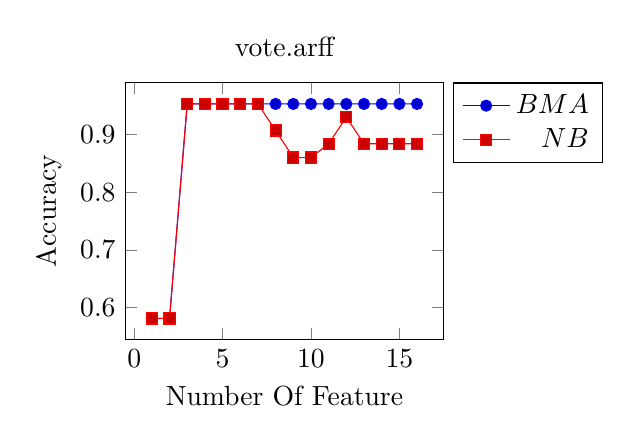
\begin{tikzpicture}%[trim axis left, trim axis right]
\begin{axis}
[title=vote.arff,
ylabel=Accuracy,
xlabel=Number Of Feature,
width=160pt,
legend style={
	cells = {anchor = east},
	legend pos = outer north east,
%	legend pos = soruh west,
	},
]
\addplot+[sharp plot] coordinates
        {(1,0.581) (2,0.581) (3,0.953) (4,0.953) (5,0.953) (6,0.953) (7,0.953) (8,0.953) (9,0.953) (10,0.953) (11,0.953) (12,0.953) (13,0.953) (14,0.953) (15,0.953) (16,0.953)};
\addplot+[sharp plot] coordinates
        {(1,0.581) (2,0.581) (3,0.953) (4,0.953) (5,0.953) (6,0.953) (7,0.953) (8,0.907) (9,0.860) (10,0.860) (11,0.884) (12,0.930) (13,0.884) (14,0.884) (15,0.884) (16,0.884)};
\legend{$BMA$,$NB$}
\end{axis}
\end{tikzpicture}
\end{center}
\caption{Example of Automatic Model Weighting and Feature Selection}
\label{figure:6}
\end{figure}
\endpgfgraphicnamed